Novel view synthesis is a fundamental problem in computer vision due to its widespread applications, such as virtual reality, augmented reality, robotics and so on. Remarkable progress has been made using neural implicit representations~\cite{NeRF2021ACM, LFN2021NIPS, SRN2019NIPS}, but these methods suffer from expensive time consumption in training and rendering~\cite{NSVF2020NIPS, FastNeRF2021ICCV, MipNeRF2021ICCV, KiloNeRF2021ICCV, PlenOctree2021CVPR, Plenoxels2022CVPR, EfficientNeRF2022CVPR, InstantNGP2022TOG}.
Recently, 3D Gaussian Splatting (3DGS)~\cite{3DGS2023ToG} has drawn increasing attention for explicit Gaussian representations and real-time rendering performance. Benefiting from rasterization-based rendering, 3DGS avoids dense points querying in scene space, so that it can maintain high efficiency and quality. 

Since 3DGS relies on per-subject~\cite{3DGS2023ToG} or per-frame~\cite{Dynamic3DGS2023arXiv} parameter optimization, several generalizable methods~\cite{GPSGaussian2023arXiv, MVSplat2024arXiv, pixelSplat2023arXiv, SplatterImage2023arXiv} are proposed to directly regress Gaussian parameters with feed-forward networks. 
Typically, these methods~\cite{MVSplat2024arXiv, pixelSplat2023arXiv} generate pixel-aligned Gaussians with U-Net architectures, epipolar transformers or cost volume representations for depth estimation and parameter predictions, and directly combine Gaussian groups obtained from different views as scene representations.
However, such combination of Gaussians leads to superfluous representations, where the overlapped regions are covered by similar Gaussians predicted separately from multiple images. 
While a simple solution is to delete redundant Gaussians, it ignores the connection among Gaussian groups. As illustrated in Figure~\ref{fig:teaser_1}, pixelSplat~\cite{pixelSplat2023arXiv} and MVSplat~\cite{MVSplat2024arXiv} suffer from artifacts with several times as many Gaussians as ours, while the deletion of similar Gaussians hurts rendering quality. 

To tackle the challenge, we propose Gaussian Graphs to model the relations of Gaussian groups from multiple views. 
Based on this structure, we present Gaussian Graph Network (GGN), extending conventional graph operations to Gaussian domain, so that Gaussians from different views are not independent but can learn from their neighbor groups.
Precisely, we reformulate the scalar weight of an edge to a weight matrix to depict the interactions between two Gaussian groups, and introduce a Gaussian pooling strategy to aggregate Gaussians.  
Under this definition, previous methods~\cite{pixelSplat2023arXiv, MVSplat2024arXiv} can be considered as a degraded case of Gaussian Graphs without edges. 
As shown in Figure~\ref{fig:teaser_2}, our GGN allows message passing and aggregation across Gaussians for efficiency representations. 

We conduct extensive experiments on both indoor and outdoor datasets, including RealEstate10K~\cite{RealEstate10K2018} and ACID~\cite{ACID2021ICCV}.
While the performance of previous methods declines as the number of input views increases, our method can benefit from more input views. As shown in Figure~\ref{fig:teaser_3}, our model outperforms previous methods under different input settings with higher rendering quality and fewer Gaussian representations.
Our main contributions can be summarized as follows:
\begin{itemize}[leftmargin=*]
    \item We propose Gaussian Graphs to construct the relations of different Gaussian groups, where each node is a set of pixel-aligned Gaussians from an input view.
    \item We introduce Gaussian Graph Network to process Gaussian Graphs by extending the graph operations to Gaussian domain, bridging the interaction and aggregation across Gaussian groups.
    \item Experimental results illustrate that our method can generate efficient and generalizable Gaussian representations. Our model requires fewer Gaussians and achieves better rendering quality.
\end{itemize}

\begin{figure}[t]
  \centering
      \subfloat[]{{\label{fig:teaser_1}}
      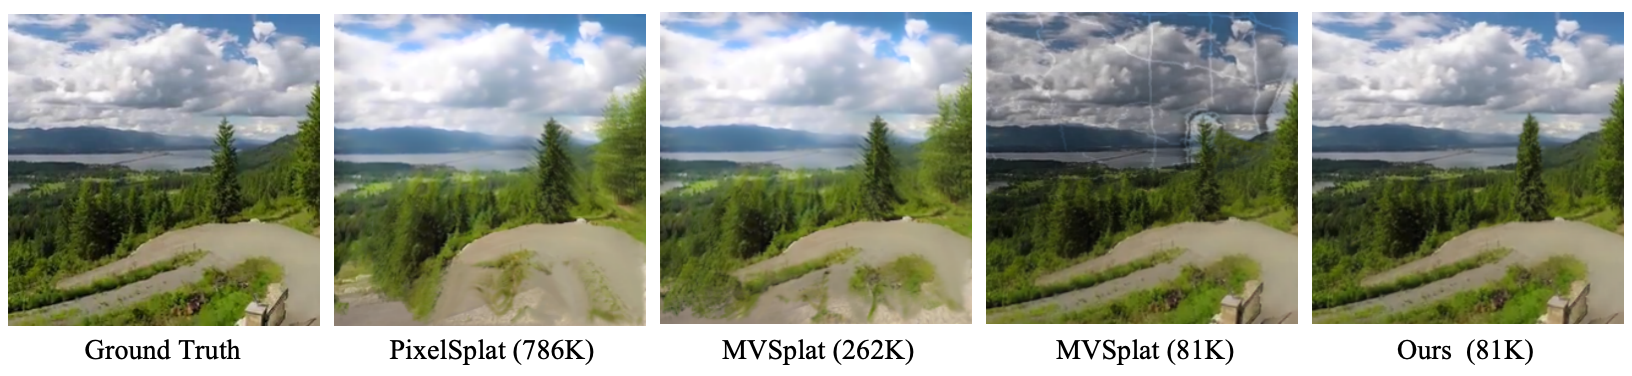
\includegraphics[height=0.22\linewidth]{fig/teaser_1.png}}
  \vspace{-0.2cm}
  \begin{minipage}[h]{0.99\linewidth}
      \centering            
      \subfloat[]{{\label{fig:teaser_2}}   
      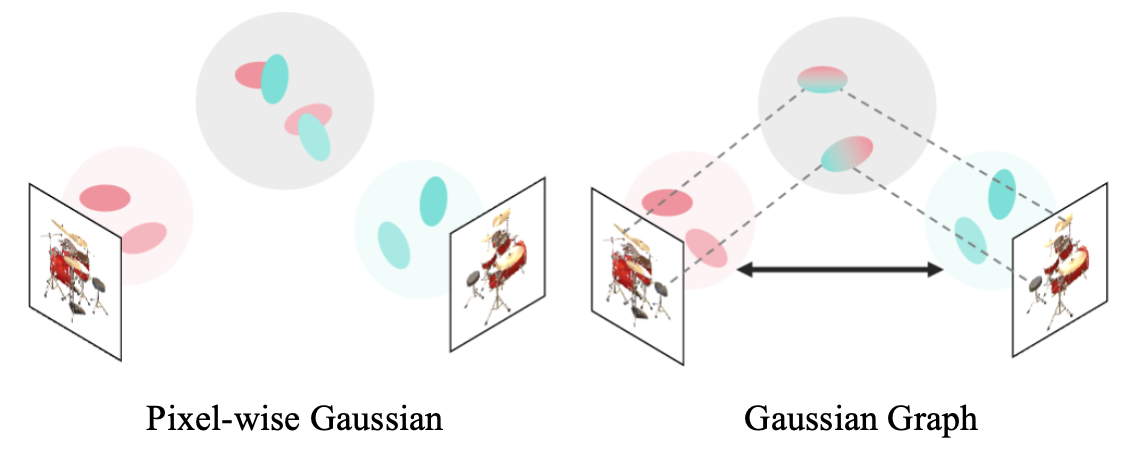
\includegraphics[height=0.26\linewidth]{fig/teaser_2.png}}
      \subfloat[]{{\label{fig:teaser_3}}
      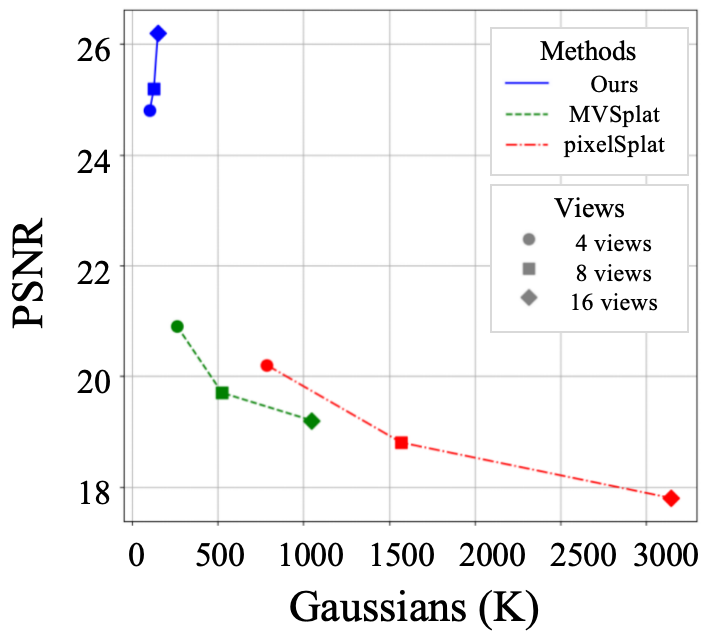
\includegraphics[height=0.26\linewidth]{fig/teaser_3.png}}
  \end{minipage}
  \caption{Comparison of previous methods and ours. (a) We visualize the rendering results of various methods and report the number of Gaussians in parentheses. (b) Previous pixel-wise methods can be considered as a degraded case of Gaussian Graphs without edges. (c) We report PSNR as well as the number of Gaussians for pixelSplat~\cite{pixelSplat2023arXiv}, MVSplat~\cite{MVSplat2024arXiv} and GNN under different input settings.}
  \label{fig:teaser}
  \vspace{-0.2cm}
\end{figure}
    
